\documentclass[compress]{beamer}
\usepackage{ifthen}

\title{Alignment Monitoring}
\author{Jim Pivarski, Dmitry Yakorev, Alexei Safonov}
\institute{Texas A\&M University}
\date{13 April, 2007}

\setbeamertemplate{navigation symbols}{}
\setbeamertemplate{headline}{\includegraphics[height=1 cm]{../cmslogo} \hspace{0.1 cm} \includegraphics[height=1 cm]{../tamulogo} \hfill
\begin{minipage}{9 cm}
\vspace{-0.75 cm} \small
\begin{center}
\ifthenelse{\equal{\insertpagenumber}{1}}{}{\insertsection}
\end{center}
\end{minipage} \hfill
\begin{minipage}{1 cm}
\vspace{-0.75 cm} \small
\begin{center}
\ifthenelse{\equal{\insertpagenumber}{1}}{}{\insertpagenumber/\pageref{numpages}}
\end{center}
\end{minipage}}

%% \xdefinecolor{verylightgray}{rgb}{0.95,0.95,0.95}
%% \beamertemplateshadingbackground{verylightgray}{white}

\begin{document}
\frame{\titlepage}
\section*{Alignment Monitoring --- Jim Pivarski}

\begin{frame}
\frametitle{Alignment monitoring: roughly four categories}
\begin{enumerate}\setlength{\itemsep}{0.4 cm}
\item DQM-based monitoring upstream of alignment process (reports an error if alignment used online is wrong)
\item \textcolor{blue}{Sanity checks in AlignmentProducer (convergence, improvement in residuals, overlap plots, $p_T$)}
\item \textcolor{blue}{Geometry Validation--- compare output geometries from different alignments: have the chambers moved?}
\item Validation with reconstructed tracks: is it better?
\end{enumerate}

\vfill Status of \textcolor{blue}{2}: Foundation for plotting modules in AlignmentProducer

\vfill Status of \textcolor{blue}{3}: Reading from multiple SQLite files, plotting difference
\end{frame}

\begin{frame}
\frametitle{Plotting Modules in AlignmentProducer (\#2)}
\begin{itemize}
\item Extends existing plugin mechanism to add monitoring modules
\end{itemize}

\vfill
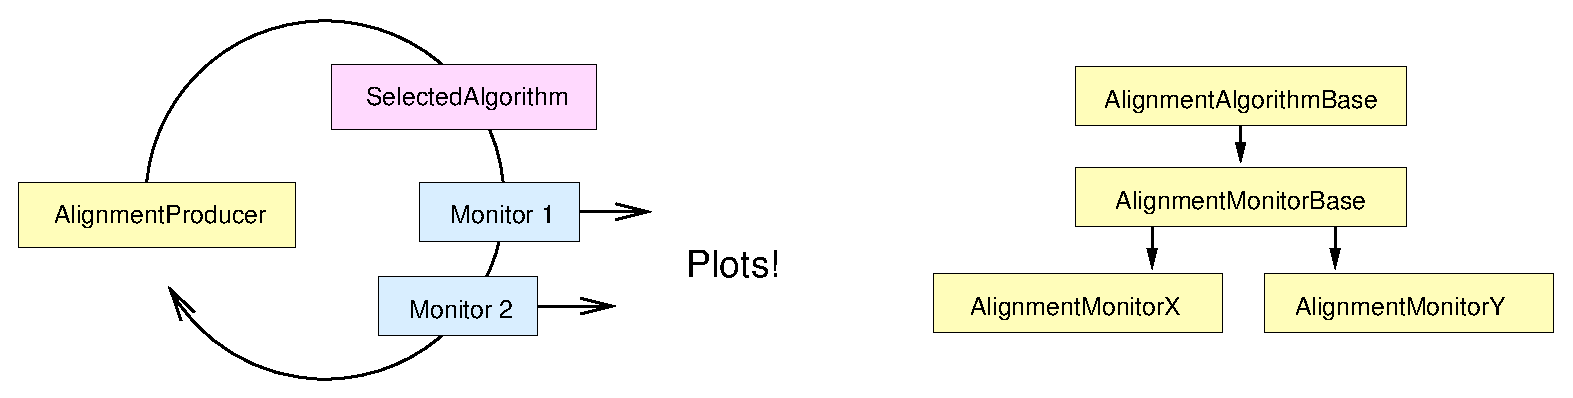
\includegraphics[width=\linewidth]{organization}

\vfill
\begin{itemize}\setlength{\itemsep}{0.25 cm}
\item Lowers ``potential barrier'' to adding plots
\item Independent of algorithm (though we can make AlignmentMonitorHIP, AlignmentMonitorMillePede, etc.)
\item Aware of iteration number, selected alignables and parameters
\item Collects and merges histograms/profiles from a distributed job
\end{itemize}
\end{frame}

\begin{frame}
\frametitle{Plotting Modules in AlignmentProducer (\#2)}

\tt \small
replace AlignmentProducer.monitorConfig = \{ \\
\mbox{\hspace{0.5 cm}}untracked vstring monitors = \{"AlignmentMonitorHIP"\} \\
\mbox{\hspace{0.5 cm}}PSet AlignmentMonitorHIP = \{ \\
\mbox{\hspace{0.5 cm}}\mbox{\hspace{0.5 cm}}string outpath = "./" \\
\mbox{\hspace{0.5 cm}}\mbox{\hspace{0.5 cm}}string outfile = "histograms.root" \\
\mbox{\hspace{0.5 cm}}\mbox{\hspace{0.5 cm}}\textcolor{gray}{bool collectorActive = false} \\
\mbox{\hspace{0.5 cm}}\mbox{\hspace{0.5 cm}}\textcolor{gray}{int32 collectorNJobs = 0} \\
\mbox{\hspace{0.5 cm}}\mbox{\hspace{0.5 cm}}\textcolor{gray}{string collectorPath = "./"} \\
\mbox{\hspace{0.5 cm}}\} \\
\}

\vfill
void AlignmentMonitorHIP::book() \{ \\
\mbox{\hspace{0.3 cm}}m\_sameForAllIters = (TH1F*)(add(\textcolor{blue}{"/"}, new TH1F(\ldots))) \\
\mbox{\hspace{0.3 cm}}m\_newForEachIter = (TH1F*)(add(\textcolor{blue}{"/iterN/"}, new TH1F(\ldots))) \\
\}
\end{frame}

\begin{frame}
\frametitle{Plotting Modules in AlignmentProducer (\#2)}
\begin{minipage}{\linewidth}
\tt \small
m\_sameForAllIters = (TH1F*)(add(\textcolor{blue}{"/"}, new TH1F(\ldots))) \\
m\_newForEachIter = (TH1F*)(add(\textcolor{blue}{"/iterN/"}, new TH1F(\ldots))) \\
\end{minipage}

\vfill
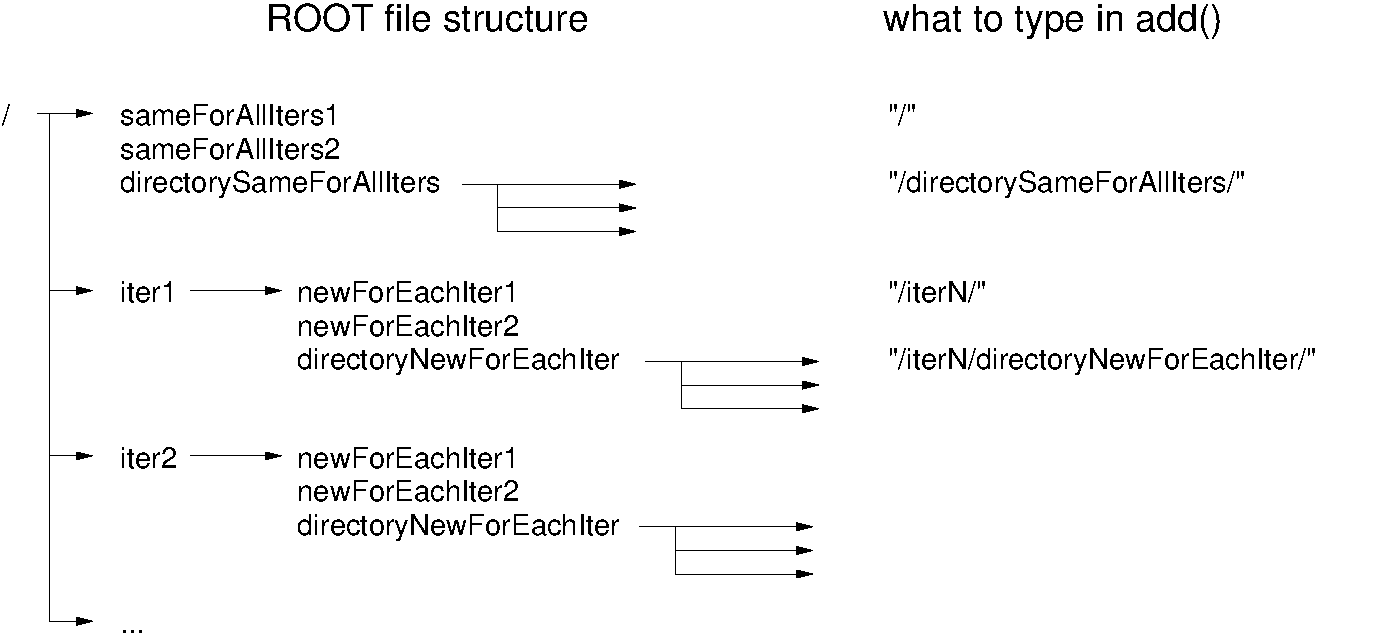
\includegraphics[width=\linewidth]{rootfile}

\vfill
Nothing more is needed for collection jobs
\end{frame}

\begin{frame}
\frametitle{Plotting Modules in AlignmentProducer (\#2)}
What works (tested for 25 events):
\begin{itemize}
  \item Loading an arbirtary number of modules
  \item Arbitrarily-deep ROOT directory structure
  \item Iteration (via {\tt AlignmentProducer.maxLoops} and/or files)
  \item Merging histograms/profiles from a distributed job
  \item Generating histograms from selected Alignables
\end{itemize}

\vfill
What's next:
\begin{itemize}
  \item Add lots of plots to AlignmentMonitorHIP
  \item Test with lots of events
  \item Put into CVS?
\end{itemize}
\end{frame}

\begin{frame}
\frametitle{Reading from multiple databases (\#3, Dmitry)}

Basic structure:
\begin{itemize}
  \item Compiled C++ ROOT GUI
  \item Forks {\tt cmsRun} processes which read SQLite files
\end{itemize}

What works:
\begin{itemize}
  \item Loading two geometry files
  \item Calculating and displaying translation differences
  \item Tabs to switch between plots
\end{itemize}

\vfill
What's next:
\begin{itemize}
  \item Read from multiple databases--- plot versus time
  \item Represent differences in rotation angles
  \item A different framework?  DQM?  Iguana?  Compile database access into ROOT GUI?
\end{itemize}
\end{frame}

\begin{frame}
\frametitle{Reading from multiple databases (\#3, Dmitry)}
\begin{columns}
\column{0.03\linewidth}
vs.\ $R$ \\

\vspace{1 cm}
vs.\ $\phi$ \\

\vspace{1 cm}
vs.\ $Z$ \\
\column{0.98\linewidth}
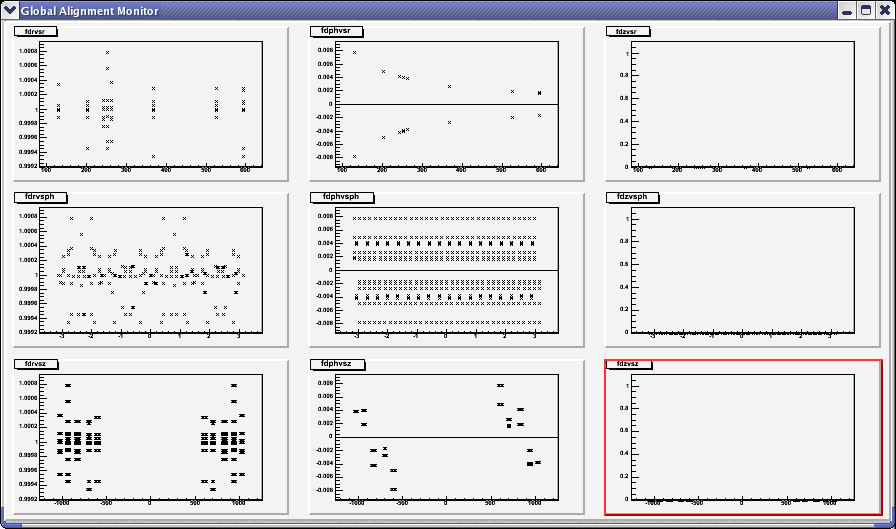
\includegraphics[width=\linewidth]{screen_shot.png}
\end{columns}

\vfill
\hfill $(\vec{x_1}-\vec{x_2})$ \hfill $(\vec{x_1}-\vec{x_2})\cdot\hat{\phi}$ \hfill $(\vec{x_1}-\vec{x_2})\cdot\hat{Z}$ \hfill
\end{frame}

\begin{frame}
\frametitle{Summary}
\begin{enumerate}\setcounter{enumi}{1}
\item \textcolor{blue}{Sanity checks in AlignmentProducer (convergence, improvement in residuals, overlap plots, $p_T$)}
\end{enumerate}

Laid a foundation that handles multiple modules, ROOT directory
structure with iterations, merging histograms after parallel processing

\vfill \vfill

\begin{enumerate}\setcounter{enumi}{2}
\item \textcolor{blue}{Geometry Validation--- compare output geometries from different alignments: have the chambers moved?}
\end{enumerate}

Measuring geometry differences across multiple SQLite files, beginnings of a GUI tool

\label{numpages}
\end{frame}

\end{document}
